\chapter{Descripci\'on del Corpus}\label{chapter:proposal}
El presente cap\'itulo describe en detalle la propuesta desarrollada para la construcci\'on de un corpus de datos no tabulares con 
atributos protegidos anotados. En la Secci\'on~\ref{section:annotation_scheme} se presenta el esquema de 
anotaci\'on dise\~nado, especificando los atributos protegidos considerados y los valores definidos para cada uno. La
Secci\'on~\ref{section:annotation_process} explica el proceso de anotaci\'on llevado a cabo, incluyendo la evaluaci\'on del 
mismo, las directrices provistas a los anotadores y las herramientas desarrolladas para facilitar el proceso. En la
Secci\'on~\ref{section:corpus_stats} se resumen las principales estad\'isticas del corpus resultante. Finalmente, en la 
Secci\'on~\ref{section:baseline} se describen dos \emph{baselines} propuestos sobre el corpus.

\section{Esquema de anotaci\'on}\label{section:annotation_scheme}
%Hablar de que cada elemento a anotar es un texto, no una sola oracion.ok
%Hablar de cuales son los atributos protegidos que se anotaron. ok
%Hablar de los valores de cada atributo protegido y mas cosas relacionadas.ok/2
En el proceso de construcci\'on del corpus, cada elemento a anotar es un texto completo que puede estar formado por varias oraciones. 
Este enfoque permite capturar el contexto completo en el que se producen las menciones a los atributos protegidos, lo cual es fundamental
para lograr una comprensi\'on m\'as precisa y contextualizada de los mismos.

En este caso, los atributos protegidos que se van a anotar son el g\'enero y la raza.
Fueron seleccionados estos atributos no solo por su relevancia en diversas \'areas de estudio y aplicaci\'on, sino tambi\'en 
por la naturaleza de los textos que se van a anotar. Dado que las rese\~nas de pel\'iculas y series de televisi\'on
pueden contener un amplia gama de discusiones sobre actores, directores y personajes, es muy probable que se pueda hacer una 
asociaci\'on con los atributos de esos individuos.

Para el atributo g\'enero los valores a anotar son: ``\emph{Male}'' para g\'enero masculino, ``\emph{Female}'' para g\'enero femenino, 
``\emph{Male, Female}'' cuando se detectan ambos g\'eneros y ``\emph{Null}'' en caso de no detectar ninguno.

En cuanto a la raza, los valores a anotar son: ``\emph{White}'' para raza blanca, ``\emph{Black}'' para raza negra, ``\emph{Indian}'' para 
personas originarias de la India, ``\emph{Arab}'' para personas de origen \'arabe, que incluye a pa\'ises del medio oriente y el norte de 
\'Africa. Adem\'as se incorpora el valor ``\emph{Latino}'' para personas de origen latinoamericano, ``\emph{Native American}'' para personas 
originarias de los pueblos nativos de Am\'erica del Norte y ``\emph{Asian}'' para personas asi\'aticas. Al igual que con el g\'enero, 
``\emph{Null}'' indica que no se detecta ninguna raza en el texto. N\'otese que, en caso de ser necesario la anotaci\'on de la raza de un 
texto puede incluir m\'as de un valor.

\section{Proceso de anotaci\'on}\label{section:annotation_process}
El proceso de anotaci\'on comienza con la selecci\'on de los textos a anotar. Inicialmente se contaba con un conjunto de $70$ textos 
extra\'idos de rese\~nas de pel\'iculas de ImDb\footnote{\url{https://www.imdb.com/}}, previamente anotados con g\'enero, producto 
de una tesis del grupo de investigaci\'on. A esta selecci\'on se a\~naden $80$ textos m\'as, extra\'idos de la misma fuente, con el 
objetivo de aumentar el tama\~no y la diversidad del corpus. Los nuevos textos se seleccionan de manera aleatoria.

Una vez seleccionados los textos, se procede a la anotaci\'on de los atributos protegidos. Esta etapa se divide en tres fases 
fundamentales:

\begin{enumerate}
    \item Anotaci\'on exhaustiva de ambos atributos por parte de dos anotadores no expertos en la problem\'atica, generando as\'i dos 
    anotaciones independientes. Los anotadores tienen permitido intercambiar opiniones y consultar dudas con un anotador experto, 
    pero no deben discutir los textos espec\'ificos que anotan.
    \item Mezcla autom\'atica de las anotaciones independientes. En caso de detectarse conflicto, un anotador experto se encarga de 
    escoger la anotaci\'on m\'as acertada. Esta etapa es asistida por \emph{scripts} de mezcla que detectan y resaltan autom\'aticamente
    los conflictos.
    \item Revisi\'on del resultado final por parte de un anotador experto, en busca de posibles errores e inconsistencias.
\end{enumerate}

Luego de estas tres fases, el conjunto de textos resultante de mezclar y revisar ambas anotaciones manuales, constituye el corpus, el 
cual debe ser evaluado como se describe en la Secci\'on~\ref{subsection:annotation_evaluation}.

\subsection{Evaluaci\'on de la anotaci\'on}\label{subsection:annotation_evaluation}
Se sugiere calcular un \emph{micro-agreement} y un \emph{macro-agreement} para evaluar el grado de concordancia entre las anotaciones
manuales del corpus. Adem\'as, se propone estudiar la consistencia estad\'istica de las anotaciones, mediante el c\'alculo  
de media, varianza y desviaci\'on est\'andar de los acuerdos entre anotadores, para cada atributo protegido.

La evaluaci\'on anterior puede ser realizada en dos fases. En la primera fase, se realiza la comparaci\'on entre las anotaciones 
realizadas por los anotadores no expertos. Luego, en la segunda fase, se comparan las anotaciones de los 
no expertos con el resultado de la mezcla y revisi\'on por parte del anotador experto. En la Secci\'on~\ref{section:results} 
se muestran los resultados obtenidos en la evaluaci\'on del corpus.

Primero se define una m\'etrica $\mathcal{J}_{attr}(A, B) \in [0,1]$, conocida como \emph{coeficiente de Jaccard}. Dicha m\'etrica 
determina para un texto el grado de concordancia entre sus dos anotaciones $A$ y $B$ de un atributo protegido $attr$, adem\'as, 
considera coincidencia parcial entre las anotaciones. Se calcula:

\begin{equation}
    \mathcal{J}_{attr}(A, B) = \frac{|A \cap B|}{|A \cup B|} = \begin{cases}
        1, & \text{si coinciden ex\'actamente} \\
        0, & \text{si la intersecci\'on es vac\'ia} \\
        0 < p < 1, & \text{en otro caso}
    \end{cases}
\end{equation}

Se define el conjunto $C_{attr} = \{\mathcal{J}_{attr}(A, B) \mid \forall (A, B)\}$. Para analizar la consistencia estad\'istica 
de las anotaciones, se calcula la media, varianza y desviaci\'on est\'andar de los conjuntos $C_{g\acute{e}nero}$ y $C_{raza}$.

Para calcular el \emph{micro-agreement}, se realiza la uni\'on de las anotaciones de ambos atributos protegidos, obteniendo as\'i
el conjunto $C_{g\acute{e}nero, raza} = \{\mathcal{J}_{attr}(A, B) \mid \forall (A, B)\}$. Luego, se calcula la media, varianza y
desviaci\'on est\'andar del conjunto obtenido. Estos resultados son una medida detallada de la concordancia en t\'erminos puntuales.
Se muestran en la Secci\'on~\ref{section:results}.

Por otra parte, la m\'etrica \emph{macro-agreement} se calcula como la media de los \emph{micro-agreements} de cada atributo protegido. 
Esta m\'etrica ofrece una perspectiva m\'as general de la concordancia entre las anotaciones, y permite detectar desbalance entre 
el \emph{agreement} por cada clase de los atributos protegidos. Se muestran en la Secci\'on~\ref{section:results}.

\subsection{Directrices de anotaci\'on}\label{section:annotation_guidelines}
%Hablar que para anotar cierto atributo no hacer falta que el texto lo mencione explicitamente, sino que se puede inferir
%Ejemplo las entidades nombradas
La caracter\'istica m\'as importante de este modelo de anotaci\'on es que busca capturar cualquier tipo de referencia a los atributos 
protegidos que se anotan. Por lo tanto, la anotaci\'on no se limita \'unicamente a menciones expl\'icitas de estos atributos en el 
texto, sino que tambi\'en se extiende a situaciones donde la referencia a g\'enero y raza puede ser inferida. La inferencia puede 
basarse en diversos elementos del texto, por ejemplo, entidades nombradas y pronombres. En caso de ser necesario el anotador podr\'a
auxiliarse de informaci\'on externa, como la b\'usqueda de im\'agenes de los personajes mencionados en el texto.

\subsection{Herramientas de anotaci\'on}
%Describir los scripts que se hicieron para anotar, mezclar y todo eso
Se desarrollaron dos \emph{scripts} de \emph{Python} para asistir en el proceso de anotaci\'on. Un primer \emph{script}
se encarga de guiar al anotador en todo este proceso, mostrando los textos a anotar y permitiendo la selecci\'on de los valores
que correspondan a cada atributo protegido. El segundo \emph{script} se encarga de mezclar las anotaciones de los anotadores 
no expertos, resaltando los conflictos y permitiendo la selecci\'on de la anotaci\'on m\'as acertada por parte del experto. 
Ambos \emph{scripts} almacenan continuamente las anotaciones en archivos \emph{CSV} para evitar posibles p\'erdidas de 
informaci\'on en caso de que ocurra alg\'un error.

\section{Estad\'isticas del Corpus}\label{section:corpus_stats}
El corpus fue construido a partir un fichero \emph{CSV}, tomado de la plataforma 
Kaggle\footnote{\url{https://www.kaggle.com/datasets/mantri7/imdb-movie-reviews-dataset}}. 
Este fichero contiene $24\,904$ rese\~nas de pel\'iculas en idioma ingl\'es. Cada entrada del fichero contiene el texto de la rese\~na, 
y un atributo binario anotado que indica si la rese\~na es positiva o negativa. Se contaba inicialmente con un conjunto de $70$ textos 
preseleccionados, a los que se a\~nadieron $80$ nuevos textos seleccionados de manera aleatoria.

Usando este conjunto de textos, se implement\'o un proceso de anotaci\'on para etiquetar manualmente el g\'enero y la raza seg\'un 
el modelo descrito en la Secci\'on~\ref{section:annotation_scheme}. Este proceso de anotaci\'on se describe en detalle en la 
Secci\'on~\ref{section:annotation_process}. La Figura~\ref{fig:ann_proc} ilustra el procesamiento realizado.
Luego del proceso de anotaci\'on, se obtuvo un total de $150$ textos anotados con g\'enero, raza y sentimiento, que constituyen el 
corpus final. Las Tablas~\ref{table:stats}, \ref{table:stats_gen} y \ref{table:stats_race}  resumen las estad\'isticas fundamentales 
del corpus final.

\begin{figure}[htpb]
    \begin{center}
        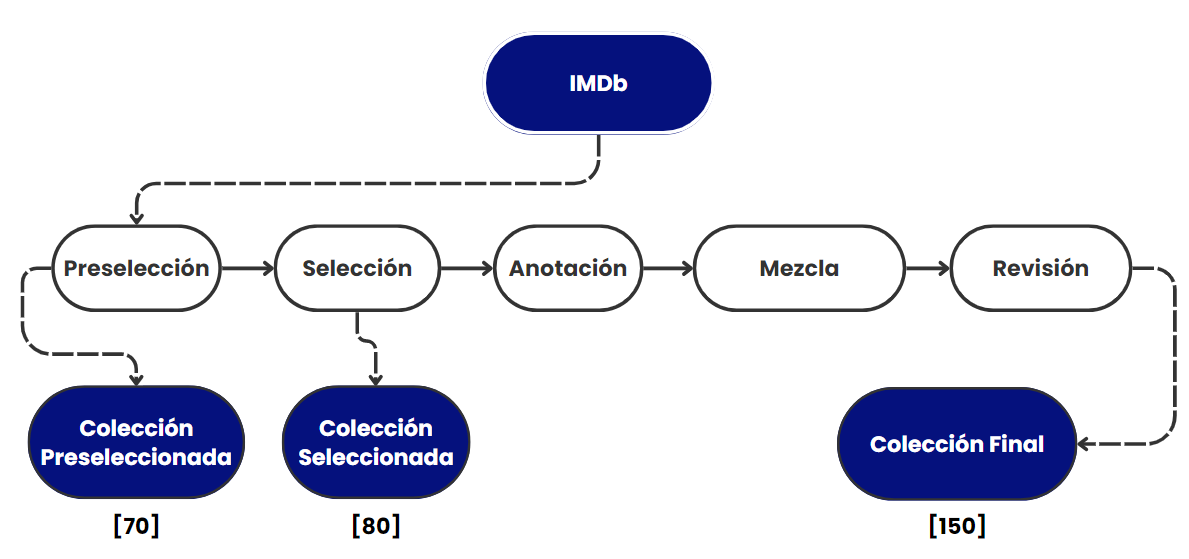
\includegraphics[width=0.8\textwidth]{Graphics/annotation_proc.png}
    \end{center}
    \caption{Representaci\'on esquem\'atica del proceso de anotaci\'on.}
    \label{fig:ann_proc}
\end{figure}

\begin{table}[htpb]
    \centering
        \begin{tabular}{lc}
        \toprule
        \textbf{M\'etrica} & \textbf{Total} \\
        \midrule
                    Textos & 150 \\
          G\'enero Anotado & 122 \\
              Raza Anotada & 107 \\

        \bottomrule
        \end{tabular}
    \caption{Resumen de las estad\'isticas generales del corpus: cantidad total de textos, cantidad de textos con g\'enero anotado y 
    cantidad de textos con raza anotada.}
    \label{table:stats}
\end{table}

\begin{table}[htpb]
    \centering
        \begin{tabular}{lc}
        \toprule
          \textbf{Clase} & \textbf{Total} \\
        \midrule
                    Male & 102 \\
                  Female & 83 \\

        \bottomrule
        \end{tabular}
    \caption{Resumen de las estad\'isticas del corpus relacionadas con el atributo g\'enero: cantidad de textos por g\'enero.}
    \label{table:stats_gen}
\end{table}

\begin{table}[htpb]
    \centering
        \begin{tabular}{lc}
        \toprule
            \textbf{Clase} & \textbf{Total} \\
        \midrule
                     White & 87 \\
                     Black & 17 \\
                     Asian & 7 \\
                    Latino & 6 \\
                    Indian & 6 \\
                      Arab & 2 \\
           Native American & 1 \\

        \bottomrule
        \end{tabular}
    \caption{Resumen de las estad\'isticas del corpus relacionadas con el atributo raza: cantidad de textos por raza.}
    \label{table:stats_race}
\end{table}

\section{Baselines}\label{section:baseline}
Uno de los objetivos del modelo de anotaci\'on propuesto en este trabajo es que pueda ser aprendido 
y replicado por una computadora. En esta secci\'on, se describe un sistema para la extracci\'on
autom\'atica de los atributos protegidos g\'enero y raza desde texto plano. Para ello, se 
implementan dos \emph{baselines}, descritos en las Secciones~\ref{subsection:ml_baseline} 
y~\ref{subsection:human_baseline}.

\subsection{Baseline de Aprendizaje Autom\'atico}\label{subsection:ml_baseline}
Este \emph{baseline} consiste en un clasificador \emph{Multilabel}  que predice 
de manera autom\'atica el g\'enero y la raza en textos de prop\'osito general, utilizando el corpus construido 
para su entrenamiento y evaluaci\'on. Esto permite determinar la capacidad de un anotador autom\'atico para 
extraer los atributos protegidos de los textos. Los resultados son discutidos en la Secci\'on~\ref{section:results}.

\subsubsection{Arquitectura del Baseline}
%parrafo de preprocesamiento
%parrafo de prediccion (los modelos de sklearn)
El preprocesamiento realizado en este caso se basa en obtener representaciones vectoriales sem\'anticas 
de los textos. Para ello, se utiliza el \emph{tokenizador} y modelo 
\emph{BERT}\footnote{\url{https://huggingface.co/docs/transformers/model_doc/bert}} preentrenados de 
\emph{Hugging Face}\footnote{\url{https://huggingface.co}}. Primero, el texto se \emph{tokeniza} con el 
\emph{tokenizador} de \emph{BERT}, convirtiendo a min\'usculas si el modelo lo requiere. Se agregan los 
\emph{tokens} especiales [CLS] y [SEP] para indicar el inicio y fin del texto respectivamente.
Luego, el texto \emph{tokenizado} se pasa a trav\'es del modelo \emph{BERT} para obtener el vector de 
\emph{embeddings} del \emph{token} [CLS], que codifica la representaci\'on sem\'antica de toda la secuencia. 

Se probaron varios modelos de clasificaci\'on supervisada brindados por la biblioteca 
\emph{sklearn}\footnote{\url{https://scikit-learn.org/}} para la predicci\'on de g\'enero y raza 
a partir de las representaciones de texto generadas por \emph{BERT}. Los modelos utilizados para 
entrenar y evaluar el clasificador fueron: \emph{Logistic Regression}, 
\emph{Random Forest Classifier}, \emph{Support Vector Machine} (SVC) y \emph{Multilayer Perceptron} (MLP).
Los resultados de cada uno se discuten en la Secci\'on~\ref{section:results}.

\subsubsection{Detalles de implementaci\'on}

En el proceso de obtenci\'on de las representaciones vectoriales de los textos, se presenta el caso
de textos que superaban el tama\~no m\'aximo de entrada admitido por \emph{BERT}, que es de $512$ \emph{tokens}.
Esto se debe a que algunos textos del corpus son rese\~nas bastante extensas. Para solucionar este problema en 
los casos que se requiera, se divide el texto en segmentos que no superen los $512$ \emph{tokens}. Luego, se obtiene
la representaci\'on vectorial de cada segmento y se promedian para obtener un \'unico vector de \emph{embedding}
representativo de todo el texto original.

\subsubsection{Hiperpar\'ametros}
Se configuraron los seguientes hiperpar\'ametros para cada uno de los modelos entrenantes utilizados:
\begin{itemize}
    \item \emph{Logistic Regression}: \emph{max\_iter} = $1\,000$
    \item \emph{Random Forest Classifier}: \emph{n\_estimators} = $100$
    \item \emph{Support Vector Machine}: todos los valores por defecto.
    \item \emph{Multilayer Perceptron}: \emph{hidden\_layer\_sizes} = ($100$, $50$), \emph{max\_iter} = $1\,000$
\end{itemize}


\subsection{Baseline Humano}\label{subsection:human_baseline}
Para complementar el \emph{baseline} de aprendizaje autom\'atico, se propone un \emph{baseline} 
basado en anotaciones realizadas por humanos. El objetivo es comparar el desempe\~no del 
clasificador contra la habilidad de anotaci\'on humana, y as\'i 
determinar qu\'e tan cerca o lejos est\'a el modelo de igualar la capacidad humana en 
esta tarea.

Es importante destacar que este \emph{baseline} no implica entrenar un modelo. En cambio,
consiste en utilizar las anotaciones realizadas por los anotadores humanos como modelo de 
clasificaci\'on. De modo que, si se requiere la predicci\'on de este clasificador para un texto, 
esta corresponda a la anotaci\'on previamente realizada por el humano.

La idea detr\'as de esto es establecer una estimaci\'on optimista de la habilidad humana en
la tarea, ya que el corpus sobre el que se realiza la evaluaci\'on fue construido precisamente 
mezclando y revisando las anotaciones humanas. En la pr\'actica, es de esperar que 
anotadores humanos sin entrenamiento espec\'ifico rindan peor que este \emph{baseline}.